\chapter{Minimum Spanning Tree - MST}
\paragraph*{INPUT}: Grafo connesso non orientato pesato $G=(V,E)$ con:\\
$W:E \rt R^+$ tale che $W(u,v)$ è il peso dell'arco (u,v).
\paragraph*{OUTPUT}: $T \subseteq E$ aciclico tale che:
\begin{enumerate}
    \item $\forall v \in V, \exists (u,v) \in T$
    \item $W(T) = \sum_{(u,v)\in T} W(u,v)$ è minimo
\end{enumerate}
$G_T = (V,T) \rt$ Minimum Spanning Tree (MST).
\begin{center}
    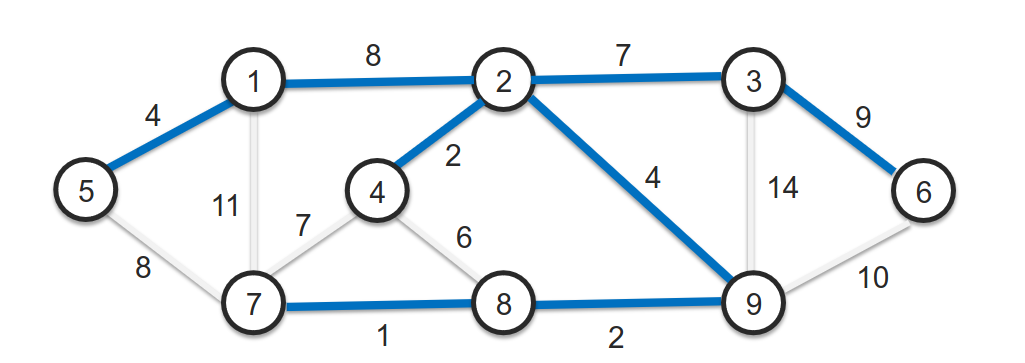
\includegraphics[width=80mm,scale=0.5]{minimum_spanning_tree.png}
\end{center}
$W(T)=37$
\section{Soluzione Generica}
\paragraph*{Algoritmo Generico}
\begin{enumerate}
    \item Inizializza un insieme A vuoto
    \item Aggiunge ad ogni passo un arco (u,v) in modo tale che $A \cup \{(u,v)\}$
    è sottoinsieme dell'insieme T degli archi MST
    \item L'algoritmo termina non appena $A=T$ (cioè, $G_A=(V,T)$ è MST)
\end{enumerate}
$(u,v)$ \ra arco sicuro per A (cioè appartiene a MST)
\begin{lstlisting}[language=Java, escapeinside={@*}{*@}]
    Procedura Generic_MST(G,W)
        A = @*\empt*@
        while @*$G_A = (V,A) \neq$*@ MST do
            trova arco (u,v) sicuro per A
            A = A @*$\cup$*@ {(u,v)}
        return A
\end{lstlisting}
\section{Definizioni Principali}
\subsection{Taglio}
\definizione{Definizione di Taglio: Partizione di V in due insiemi $V'$ e $V-V'$}
\subsection{Arco che Attraversa il Taglio}
\definizione{Definizione di Arco che \underline{Attraversa} il Taglio: arco $(u,v) \in E$ tale che u appartiene a $V'$ e v 
appartiene a $V'-V$} 
\paragraph*{Esempio di Taglio}
\begin{center}
    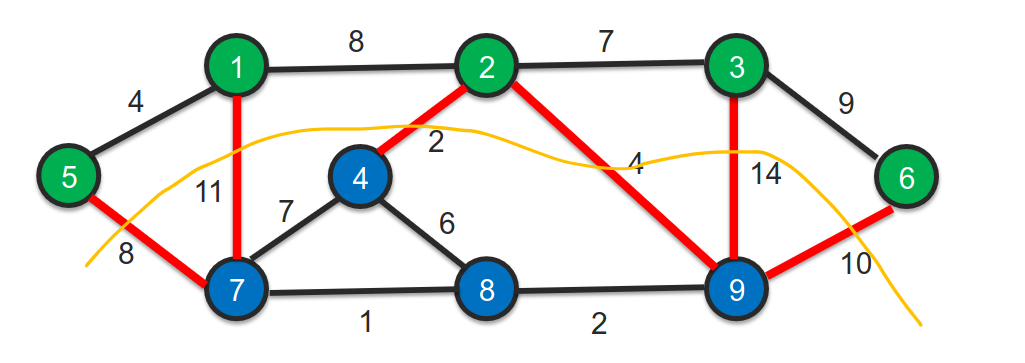
\includegraphics[width=80mm,scale=0.5]{mst_taglio.png}
\end{center}
$V' = \{1,2,3,5,6\}$\\
$V'-V=\{4,7,8,9\}$\\
\subsection{Taglio che rispetta un insieme}
\definizione{Un taglio che \underline{rispetta} un insieme $A \subseteq E$, se nessun arco di A
attraversa il taglio}
\begin{center}
    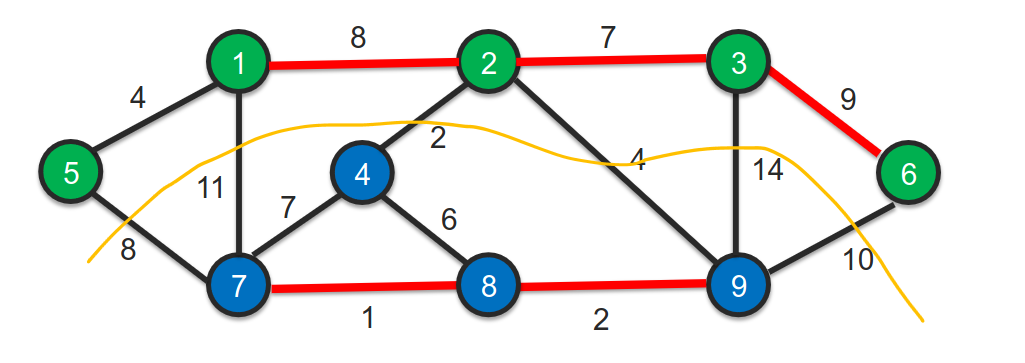
\includegraphics[width=80mm,scale=0.5]{mst_taglio_rispetta.png}
\end{center}
Il taglio rispetta $A = \{(1,2),(2,3),(3,6),(7,8),(8,9)\}$.
\subsection{Arco Leggero}
\definizione{Arco di peso minimo che attraversa il taglio}
\begin{center}
    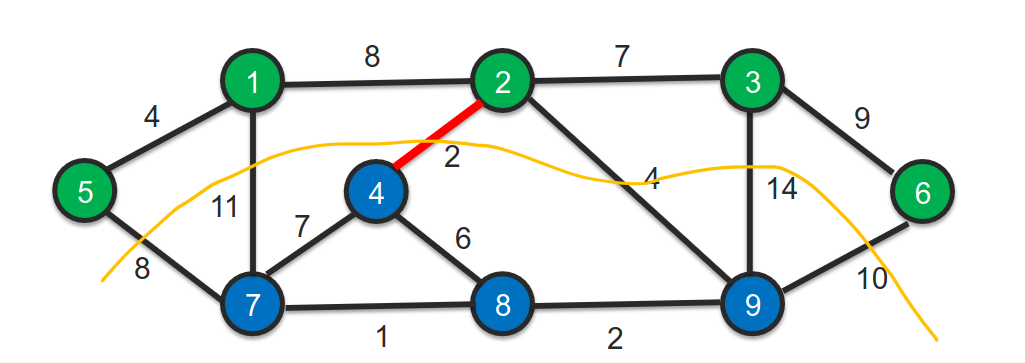
\includegraphics[width=80mm,scale=0.5]{mst_taglio_leggero.png}
\end{center}
(4,2) \ra arco \underline{leggero}
\section{Teorema dell'arco sicuro}
Dati un grafo connesso non orientato e pesato $G=(V,E)$, un sottoinsieme A dell'insieme T di archi di un
Minimum Spanning Tree (MST) e un qualsiasi taglio che rispetti A, allora un arco leggero (u,v) del taglio è
sicuro per A, cioè $A \cup \{(u,v)\} \subseteq T$.
\subsection{Proof}
Considero T \ra insieme di archi di un MST.\\
$A \subseteq T \rt$ sottoinsieme di T.\\
Taglio che rispetta A = (\tikz \fill[green] (0,0) circle (2pt);, \tikz \fill[blue] (0,0) circle (2pt);).\\
$(u,v) \rt$ arco leggero del taglio.
\begin{center}
    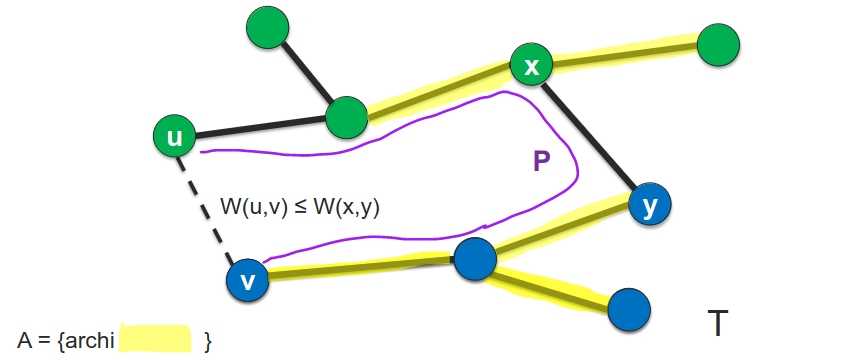
\includegraphics[width=80mm,scale=0.5]{arco_sicuro_dim_mst.png}
\end{center}
Il peso $W(u,v)$ è sicuramente $\leq$ rispetto al peso $W(x,y)$.\\
Sostituisco $(x,y)$, con $(u,v)$ e inserisco quindi l'arco $(u,v)$ all'interno
del grafo e noto che il grafo resta comunque un albero, vedo che resta un MST dato
che non ci sono cicli, ottengo quindi $T'$ con $W(T') \leq W(T)$.\\
\begin{center}
    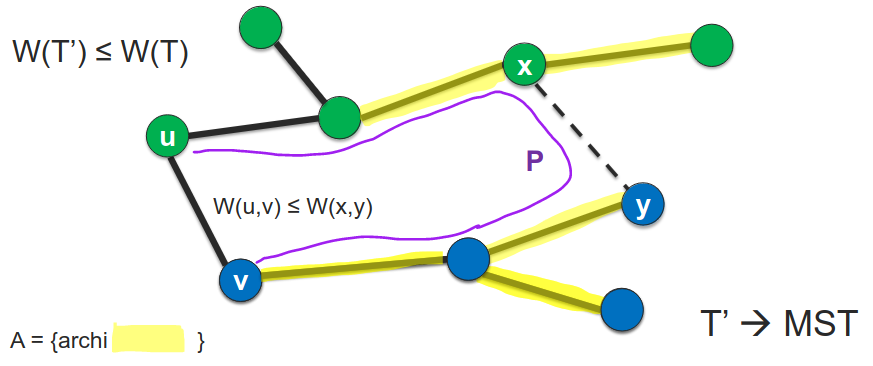
\includegraphics[width=80mm,scale=0.5]{arco_sicuro_dim_mst_2.png}
\end{center}
Per ipotesi, $A \subseteq T$ non contiene $(u,v)$ e $(x,y)$ e per costruzione $T'$ 
non contiene $(x,y)$.\\
$\implies A \subseteq T'$\\
$A \cup \{(u,v)\} \subseteq T'$
\subsection{Esempio Teorema}
Dato il seguente sottoinsieme di T denominato $A = \{archi blu\} \subseteq T$, prendiamo\\
l'arco (2,4) \ra che è arco leggero (dato che ha peso 2), posiamo dire che è un arco sicuro,
infatti se guardiamo T notiamo che $A \cup \{(2,4)\} \subseteq T$, infatti l'arco appartiene
all'MST T.
\begin{center}
    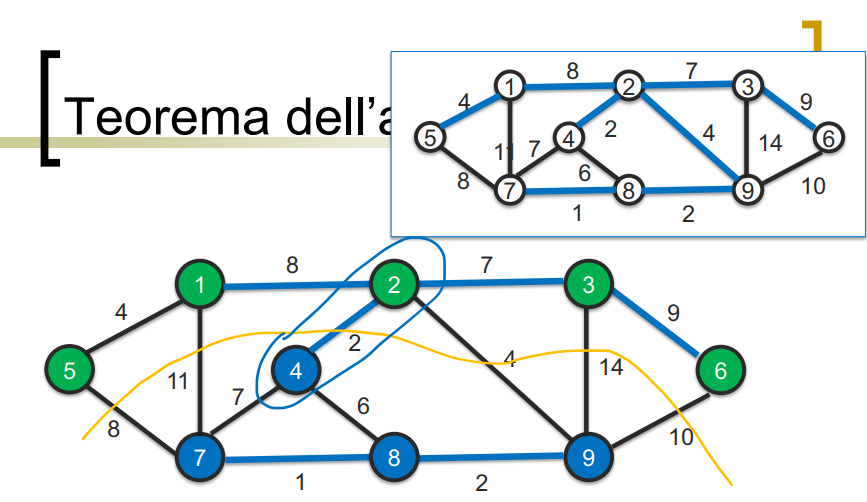
\includegraphics[width=80mm,scale=0.5]{arco_sicuro_es.png}
\end{center}
\subsection{Soluzione generica}
\begin{lstlisting}[language=Java, escapeinside={@*}{*@}]
    Procedura Generic_MST(G,W)
        A = @*\empt*@
        while @*$|V|-|A|>1$*@ do
            trova arco (u,v) sicuro per A
            A = A @*$\cup$*@ {(u,v)}
        return A
\end{lstlisting}
\begin{enumerate}
    \item A rimane aciclico durante le iterazioni
    \item $G_A = (V,A)$ (ad ogni iterazione) è una foresta di $|V|-|A|$ alberi
    \item All'inizio $G_A$ contiene $|V|$ alberti (i singoli vertici)
    \item Ogni iterazione riduce di 1 il numero di alberi e l'arco sicuro (u,v) collega
    sempre componenti distinte di $G_A$
    \item Quando si arriva a un solo albero l'algoritmo termina
    \item Il numero di iterazioni è pari a $|V|-1$
\end{enumerate}
\subsection{COROLLARIO}
$A\subseteq T$ è tale che $G_A = (V,A)$ è una foresta di $|V|-|A|$ alberi.\\
Sia $C= (V_C, A_C), V_C \subseteq V$ e $A_C \subseteq A$, una componente connessa di $G_A$\\
$\implies (V_C, V-V_C)$ è sicuramente un taglio che \underline{rispetta} A\\
$\implies$ un arco leggero di $(V_C, V-V_C)$ è arco \underline{sicuro} per A.\\
\paragraph*{QUINDI} Ad ogni iterazione, per aggiungere ad A un arco sicuro (arco di MST) basta:
\begin{enumerate}
    \item Considerare una delle componenti C della foresta $G_A = (V,A)$
    \item Trovare l'arco di peso minimo che collega un vertice in C con un vertice non in C
\end{enumerate}
\begin{center}
    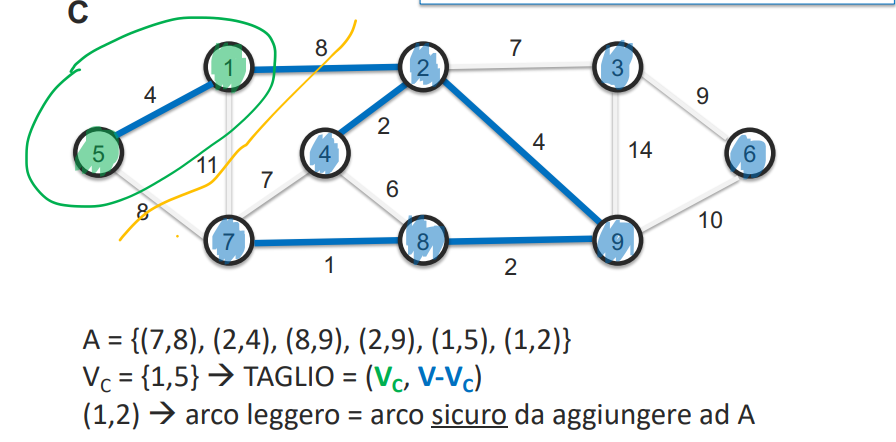
\includegraphics[width=80mm,scale=0.5]{arco_sicuro_corollario.png}
\end{center}
\paragraph*{Corollario} Dati un grafo connesso non orientato e pesato G = (V,E), un
sottoinsieme A degli archi di MST, una componente connessa $C = (V_C, E_C)$ di $G_A = (V,A)$,
allora un arco leggero (u,v) del taglio $(V_C, V-V_C)$ è un arco \underline{sicuro} per A.
\subsection{Implementazione GENERIC-MST}
Ci sono principalmente due implementazioni di GENERIC-MST e sono 2 algoritmi:
\begin{itemize}
    \item Algoritmo di Kruskal
    \item Algoritmo di Prim
\end{itemize}
\section{Algoritmo di Kruskal}
\textbf{MST = Sottoinsieme ottimo di un matroide grafico $M_G$}.
$M_G = (S,F)$ per $G=(V,E,W)$ non orientato e connesso:
\begin{itemize}
    \item S, insieme E degli archi di G
    \item F, tutti i sottoinsiemi di S che sono aciclici
\end{itemize}
pesato con:\\
$W:S \rt R^+$ tale che $W(s)$ è il peso dell'arco s.\\
Sottoinsieme ottimo di $M_G$ pesato con W\\
\ra Archi dello Spanning Tree (ST) di peso massimo.\\
$W':S \rt R^+$ tale che $W'(s) = W_0 - W(s)$\\
$W_0$ è il massimo valore del peso degli archi (massimo per W)\\
Sottoinsieme ottimo di $M_G$ pesato con $W'$\\
\ra Sottoinsieme masimale di peso massimo (per $W'$) e di peso minimo per W che equivale a dire:\\
\ra Archi dello Spanning Tree (ST) di peso \underline{minimo}, cioè l'MST.
\subsection{Algoritmo Greedy Standard per il matroide grafico}.
\begin{lstlisting}[language=Java, escapeinside={@*}{*@}]
    Procedura Generic_matroid_grafic(E = @*$\{e_1, e_2, ..., e_n\}$*@)
        X = @*$\emptyset$*@
        Ordino E per peso W crescente (non decrescente)
        for i form 1 to n do
            if @*$e_i$*@ arco sicuro then
                A = @*$\{e_i\} \cup A $*@
        return A
\end{lstlisting}
\subsection{Algoritmo Kruskal}
\begin{lstlisting}[language=Java, escapeinside={@*}{*@}]
    Procedura KRUSKAL_MST(G = (V,E), W)
        A = @*$\emptyset$*@
        E = @*$\langle e_1, e_2, ..., e_n \rangle$*@ ordinati per peso crescente (non decr.)
        for i form 1 to n do
            if @*$\{e_i\} \cup A \subseteq T$*@ then
                A = @*$\{e_i\} \cup A $*@
        return A
\end{lstlisting}
Devo tradurre in codice l'if che determina se $e_i$ è un arco sicuro e per fare questo
\textbf{applico il corollario}:\\
$e_i = (u,v)$ è arco sicuro se è un arco di peso minimo che connette un vertice di una componente C
con un vertice che non è in C. Quindi $e_i$ è arco sicuro se connette due componenti diverse
di $G_A = (V,A)$. Quindi basta asssegnare l'arco che sto analizzando $e_i$ a $(u,v)$ e se
non appartengono alla stessa componente di $G_A(V,A)$, allora posso aggiungere l'arco alla soluzione A.
\begin{lstlisting}[language=Java, escapeinside={@*}{*@}]
    Procedura KRUSKAL_MST(G = (V,E), W)
        A = @*$\emptyset$*@
        E = @*$\langle e_1, e_2, ..., e_n \rangle$*@ ordinati per peso crescente (non decr.)
        for i form 1 to n do
            (u,v) = @*$e_i$*@
            if u e v @*$\notin$*@ stessa componente di @*$G_A(V,A)$*@ then
                A = @*$\{(u,v)\} \cup A $*@
        return A
\end{lstlisting}
\subsection{Esempio di Esecuzione Algoritmo Kruskal}
\paragraph*{Passo 1} Ordina E per peso non decrescente \ra $E=\langle e_1, e_2, ..., e_m\rangle$,
in modo tale da avere nell'insieme E prima gli archi più leggeri e mano a mano quelli più
pesanti, in questo modo posso applicare un approccio Greedy.\\
Inizializza $A = \emptyset$.\\
\paragraph*{Inizio a considerare gli archi} Considero $e_1 = (7,8)$, connette due componenti di
$G_A$?
\begin{center}
    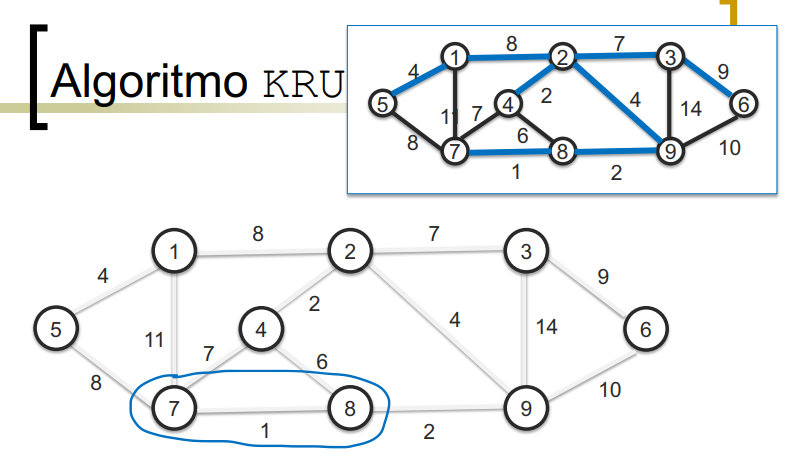
\includegraphics[width=80mm, scale=0.5]{kruskal_esec1.png}
\end{center}
Sì, quindi $\implies A = \{(7,8)\}$.\\
Considero ora il secondo arco $e_2 = (2,4)$, connette due componenti di $G_A$?
\begin{center}
    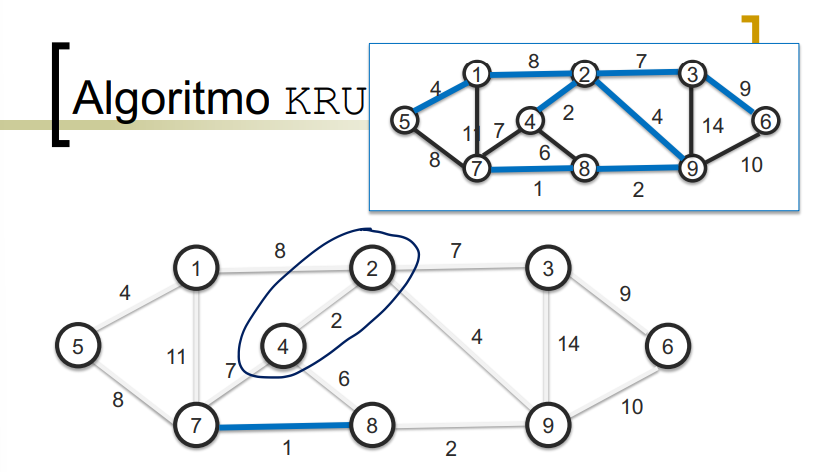
\includegraphics[width=80mm,scale=0.5]{kruskal_esec2.png}
\end{center}
Sì, quindi $\implies A = \{(7,8), (2,4)\}$.\\
Saltiamo qualche passo dove aggiungiamo sempre archi perchè troviamo sempre che
gli archi considerati connettono due componenti.\\
Consideriamo l'arco $e_6=(4,6)$
\begin{center}
    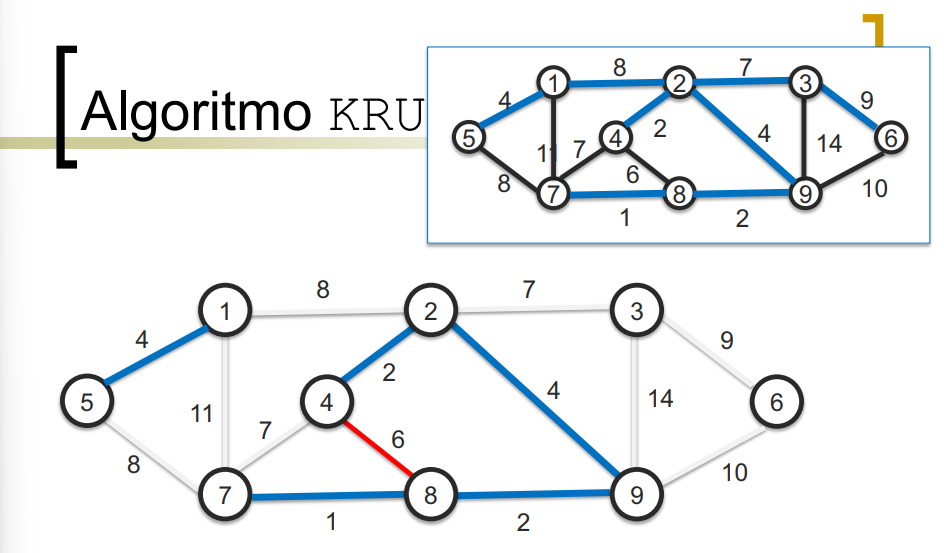
\includegraphics[width=80mm,scale=0.5]{kruskal_esec3.png}
\end{center}
Notiamo che in questo caso l'arco non connette due componenti di $G_A$ (le 
componenti sono già connesse tramite altri archi, aggiungere questo arco creerebbe
un ciclo), per questo non considero questo
arco e procedo a considerare il successivo.\\
Continuo in questo modo fino a quando non ho considerato tutti gli archi. Alla fine
avrò ottenuto l'MST!
\subsection{Codice Kruskal}
Abbiamo già scritto in precedenza il codice di Kruskal, ma come possiamo tradurre le istruzioni
matematiche in codice? Riscriviamo le parti riguardante il controllo di appartenenza al grafo.
\begin{lstlisting}[language=Java, escapeinside={@*}{*@}]
    KRUSKAL-MST(G=(V,E),W)
    A = @*$\emptyset$*@
    E = @*$\langle e_1, e_2, ..., e_n \rangle$*@ ordinati per peso crescente (non decr.)
    foreach v @*$\in$*@ V do
        MAKE_SET(V)
    for 1 from 1 to n do
        (u,v) = @*$e_i$*@
        if FIND_SET(u) @*$\neq$*@ FIND_SET(v) then
            A = @*$\{(u,v)\} \cup A $*@
    return A  
\end{lstlisting}
Tramite la strutture dati FIND SET andiamo ad analizzare se aggiungendo l'arco (u,v), otteniamo
un nuovo albero (quindi connettiamo due componenti) o se abbiamo sempre lo stesso albero (quindi non stiamo
connettendo le componenti, ma stiamo generando un ciclo). se le 2 FIND SET sono diverse allora
possiamo aggiungere l'arco alla soluzione finale tramite la UNION,
altrimenti lo scarto e passo a quello successivo.
\paragraph*{Complessità Algoritmo}
\begin{itemize}
    \item L'ordinamento degli archi avrà complessità $O(|E|\log |E|)$ (Merge Sort)
    \item il MAKE SET avrà complessità $O|V|$
    \item Mentre tutto il blocco for fino a UNION ha complessità $O(|E|\alpha)$, dove
    $\alpha$ è una funzione che cresce molto lentamente che è il tempo di aggiunta degli
    elementi tramite UNION
\end{itemize}
Avendo G connesso \ra $|E| \geq |V|-1$ che possiamo approssimare a $|E|$, quindi
$(|V|+|E|\alpha)$ sarà $(2|E|\alpha)$, ma essendo il 2 un coefficiente costante nell'utilizzo
dell'O è trascurabile.\\
In totale avrò $O(|E|\log |E|+|E|\alpha)$.\\
Sicuramente $\alpha \leq \log |V|$, perchè $\alpha$ cresce molto lentamente
$|V| = |E|$, per questo motivo avrò:\\
\paragraph*{Complessità} $O(E \log|E| + |E|\log |E|)$ quindi\\
$O(|E|\log |E|)$.

\section{Algoritmo di Prim}
Altro algoritmo utilizzato per trovare l'albero di copertura minimo in un grafo che in questo
caso si basa sull'effettuare tagli e scegliere l'arco leggero (quindi sicuro).\\
Si basa sull'assegnazione di un peso ai vertici e questo è un meccanismo utilizzato anche
da un altro algoritmo che vedremo più avanti denominato Dijkstra.
\subsection{Idea dell'algoritmo}
\begin{enumerate}
    \item Sceglie un vertice arbitrario r (componente C iniziale composta dal solo
    vertice r)
    \item Trova l'arco di peso minimo che connette r a un altro vertice v
    (il vertice v entra a far parte di C)
    \item Trova l'arco di peso minimo che connette un vertice in C a un vertice
    v non in C, (il vertice v entra a far parte di C)
    \item Etc.
    \item L'algoritmo termina quando la componente C comprende tutti i vertici
    del grafo e coincide quindi con il Minimum Spanning Tree
\end{enumerate}
\subsection{Proprietà dell'algoritmo}
Ad ogni passo:
\begin{enumerate}
    \item Il sottoinsieme A degli archi di MST aggiunti, stanno tutti nella componente C.
    La foresta $G_A = (V,A)$ è composta da:
    \begin{itemize}
        \item $C = (V_C, A)$
        \item $|V-V_C|$ componenti di vertici singoli
    \end{itemize}
    \item Il taglio $(V_C, V-V_C)$ rispetta l'insieme A
    \item l'arco sicuro è l'arco di peso minimo che connette un vertice in C con
    un vertice non in C
\end{enumerate}
L'idea è quindi quella di effettuare dei tagli tali per cui $(V_C, V-V_C)$ rispetta
l'insieme A, quindi effettuo dei tagli tra l'insieme A gli archi già aggiunti
all'MST e gli altri archi e considero l'arco leggero. Per il teorema dell'arco sicuro, 
l'arco sicuro è l'arco di peso minimo che connette un vertice in C con un vertice
non i C.
\paragraph*{Esempio} Qui di seguito notiamo che effettuando il taglio e scegliendo l'arco
leggero preleviamo automaticamente l'arco sicuro.
\begin{center}
    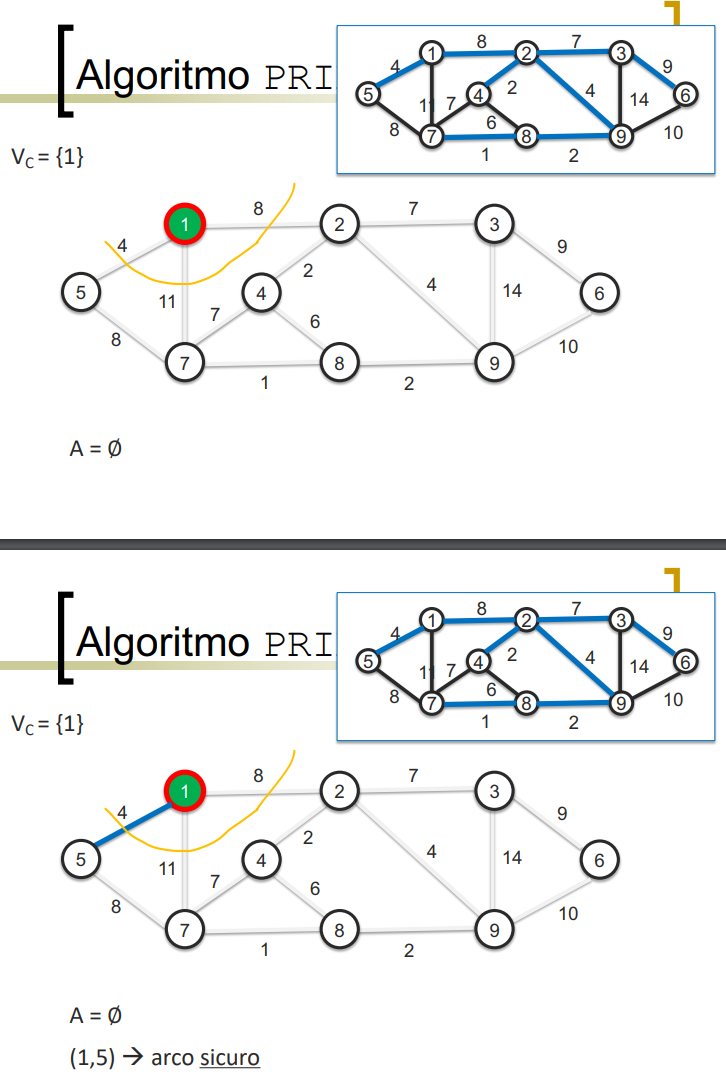
\includegraphics[width=80mm,scale=0.5]{prim_exec1.png}
\end{center}
Continuando ad effettuare tagli validi e a selezione l'arco leggero (quindi sicuro) otteniamo
otterremo l'MST.
\subsection{Implementazione Prim}
Come possiamo implementare in maniera efficiente l'esecuzione del taglio e la
conseguente ricerca dell'arco di peso minimo?\\
Assegneremo dei pesi ai vertici e un valore contenente il suo predecessore per ogni v in V e utilizzeremo
come struttura dati una \textbf{coda Q di min-priority}.\\
La \textbf{min priority queue} è coda particolare che con l'operazione di Dequeue permette
di estrarre l'elemento di priorità minima, in questo caso ci servirà per ottenere sempre l'elemento
di peso minimo.\\
Inizializziamo i pesi a infinito e i valori del predecessore a NIL:
\begin{itemize}
    \item v.key = $\infty$
    \item v.$\pi$ = NIL
\end{itemize}
Scegliamo un vertice r arbitrario, nell'esempio scegliamo $r = 1$ e peso $1.key = 0$.\\
Inseriamo tutti i vertici in una coda Q di min priority che permette l'estrazione 
del vertice con il minimo valore del campo key.
\begin{center}
    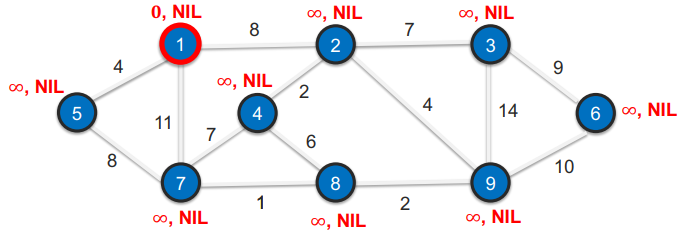
\includegraphics[width=80mm,scale=0.5]{prim_impl1.png}
\end{center}
Estraiamo ora da Q il vertice con il minimo valore di key \ra vertice 1.\\
Procediamo quindi ad esaminare gli adiacenti di 1 \ra 2, 7, 5.\\
2 appartiene a Q and $W(1,2) < 2.key \\ \implies 2.key = (1,2);\quad 2.\pi = 1$.
\begin{center}
    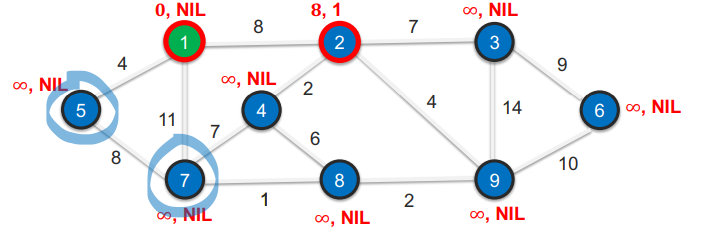
\includegraphics[width=80mm,scale=0.5]{prim_impl2.png}
\end{center}
Considero il secondo adiacente, 7. Esso appartiene a Q and $W(1,7) < 7.key \\
\implies 7.key = W(1,7);\quad 7.\pi = 1$.
\begin{center}
    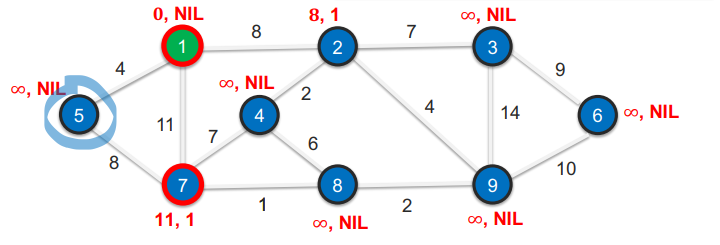
\includegraphics[width=80mm,scale=0.5]{prim_impl3.png}
\end{center}
%slide 236 Continua con l'analisi del terzo vertice adiacente 5